\chapter{Related Work}

\section{2D and 3D Visualizations}

Although the focus of this thesis is on visualizing hierarchical networks in virtual reality, many concepts are the same or similar to its 2D or 3D counterparts. So first we want to give a brief overview of related 2D and 3D approaches in the field of network visualization.\\
Dynamic network visualization describes a research field where none or only few assumptions about the data are made, the technique usually works by force-based layouts using node-link diagrams as we already summarized in the background section \ref{exp:force_based_background}. Furthermore, we want to discuss approaches dealing with hierarchical and multilayer structured datasets.

\subsection{Hierarchical Visualizations}

As we read in \ref{exp:tree} before, a preferred data structure to encode hierarchical information are trees.
Schulz \cite{schulz_treevisnet_2011} presented a good overview of different tree visualization techniques. A rough separation can be made by the representation of edges witch is either explicit or implicit. 

\subsubsection{Explicit approaches}
On explicit visualizations links are directly drawn as we have already seen in \ref{fig:simple_tree}. This core technique is used in numerous application domains and has been brought present over multiple scientific fields. Based on that concept researchers have developed many extensions.
LensTree \cite{song_lenstree_2006} for example, exchanges the axes and allows collapsing certain parts of the tree to display information structures like computer file directories. 
Armando et al. \cite{arce-orozco_radial_2017} uses radial instead of parallel axes to show the hierarchical relation, the root node is placed in the center and child nodes extend to all directions along the radius.
Munzer et al. \cite{munzner_h3_1997} extend the radial axis by a third dimension and displays the tree in the 3D hyperbolic space.
Robertson et al. \cite{robertson_cone_1991} also make use of the 3D space in his publications of the cone-tree and cam-tree, these display the child nodes as a circle below respectively beside their parents.  

\subsubsection{Implicit approaches - space filling}
The concept of nesting, which we also use in our layout, is heavenly used by space filling approaches. In addition, these usually encode the node-size into the used area as we have already seen in Figure \ref{fig:hierarchicalCirclePlot}.
Shneiderman \cite{shneiderman_tree_1992} presented this approach 1992 in the form of a tree map where he visualized the required disk space distribution of a file system. In addition to a common circle packing algorithm \ref{fig:hierarchicalCirclePlot}, Görtler \cite{gortler_bubble_2018} developed a bubble tree map technique which optimized the used space and allows encoding of additional properties via various shapes, draw strokes and colors. Sunburst charts are another common space filling technique to display node sizes in tree structures. 
As for 3D representations, Wang \cite{wang_visualization_2006} shows us a circular tree map extending to the z axis using cylinders. Instead of cylinders Balzer \cite{balzer_hierarchy_2004} uses nested hemispheres to visualize software structures.
Lastly, research is not limited to the layout of the visualization, as Itoh \cite{itoh_hierarchical_2004} shows us with their performance optimized technique for generating a rectangle packing tree map.

We can conclude that there are many approaches with various explicit and implicit layouts for tree visualizations, which focus on mapping hierarchical relationships for one network at a time. However, there are no links between multiple networks as this would mean there is a cycle in the original data and therefore breaking the definition of a tree structure in the first place. 

\subsection{Multilayer Visualization}
As we already figured out in section \ref{exp:multilayer}, the interesting part of multilayer visualizations is that it enables us to model relationships between multiple separated networks. Which was not possible with common node-link and tree visualization techniques we discussed before.\\
Domenico et al. \cite{de_domenico_muxviz_2015} presented their MuxVis Toolkit, an open-source software which is able to present multilayer datasets. In direct comparison to other approaches we have seen this one stands out as it provides a complete and user-friendly software package with various layouts (see Figure \ref{fig:muxVisExample}) like a classical stacked one-line layer, a multi-line layer where multiple stacked layer planes are displayed beside each other, a force directed method and lastly a matrix layout. Besides these called 2.5D approaches we also see some classical 2D node-links networks, for example Ducruet \cite{ducruet_multilayer_nodate} display multiple networks of different marine traffic in a single graph just coded by color. 
A combination of multilevel graphs and hierarchical information can be seen in the approach by Eades \cite{eades_multilevel_1997} et al., here the authors group the nodes into nested clusters these are then displayed with a classical multilayer approach as flat layers below each other. The difference to general multilayer graphs is that each node has exact one connection to its (parent) node in the higher layer. 
Later on, Balzer et al. \cite{balzer_level--detail_2007} (see Figure \ref{fig:clusteredGraph}) created a similar visualization but instead of flat layers they used compact 3D surfaces to cluster and group their nodes. Their approach is really similar as it also allows of nesting multiple level of nodes and clusters, however they do not have a strict hierarchical aspect. 
Jonker et al. \cite{jonker_graph_2017} uses a level of detail approach where they group parts of the graph into clusters and only display single nodes when zooming into a specific tile. With their 2D layout therefore they achieve to visualize huge networks with a couple of hundred thousand nodes and links. 

\begin{figure}[h]
    \centering
    \begin{subfigure}[b]{0.75\columnwidth}
        \centering
        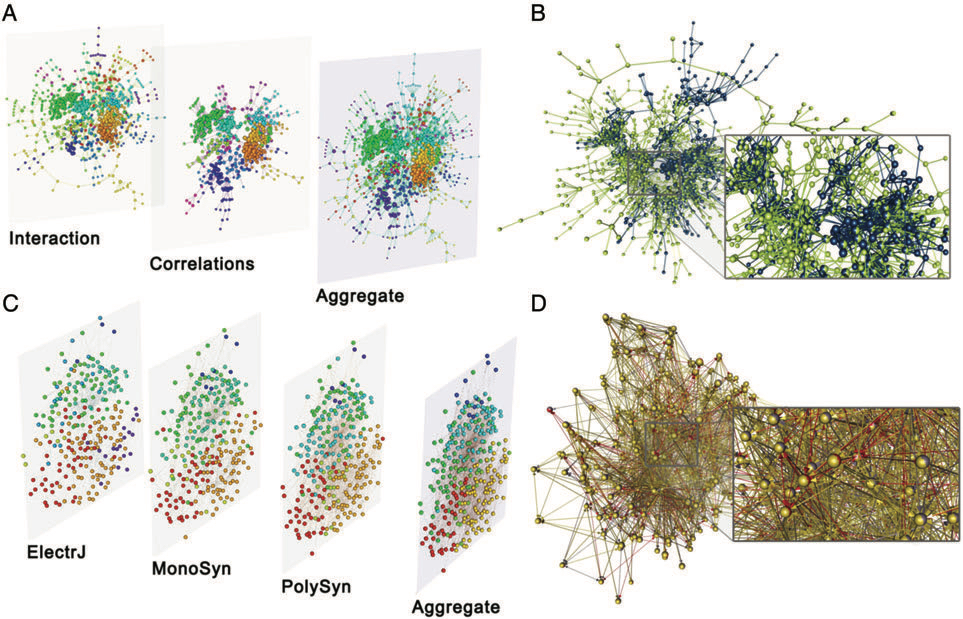
\includegraphics[width=\textwidth]{graphics/muxVisExample.jpg}
        \subcaption{Different supported layout techniques by MuxVis \cite{de_domenico_muxviz_2015}. }
        \label{fig:muxVisExample}
    \end{subfigure}
    \begin{subfigure}[b]{0.45\columnwidth}
        \centering
        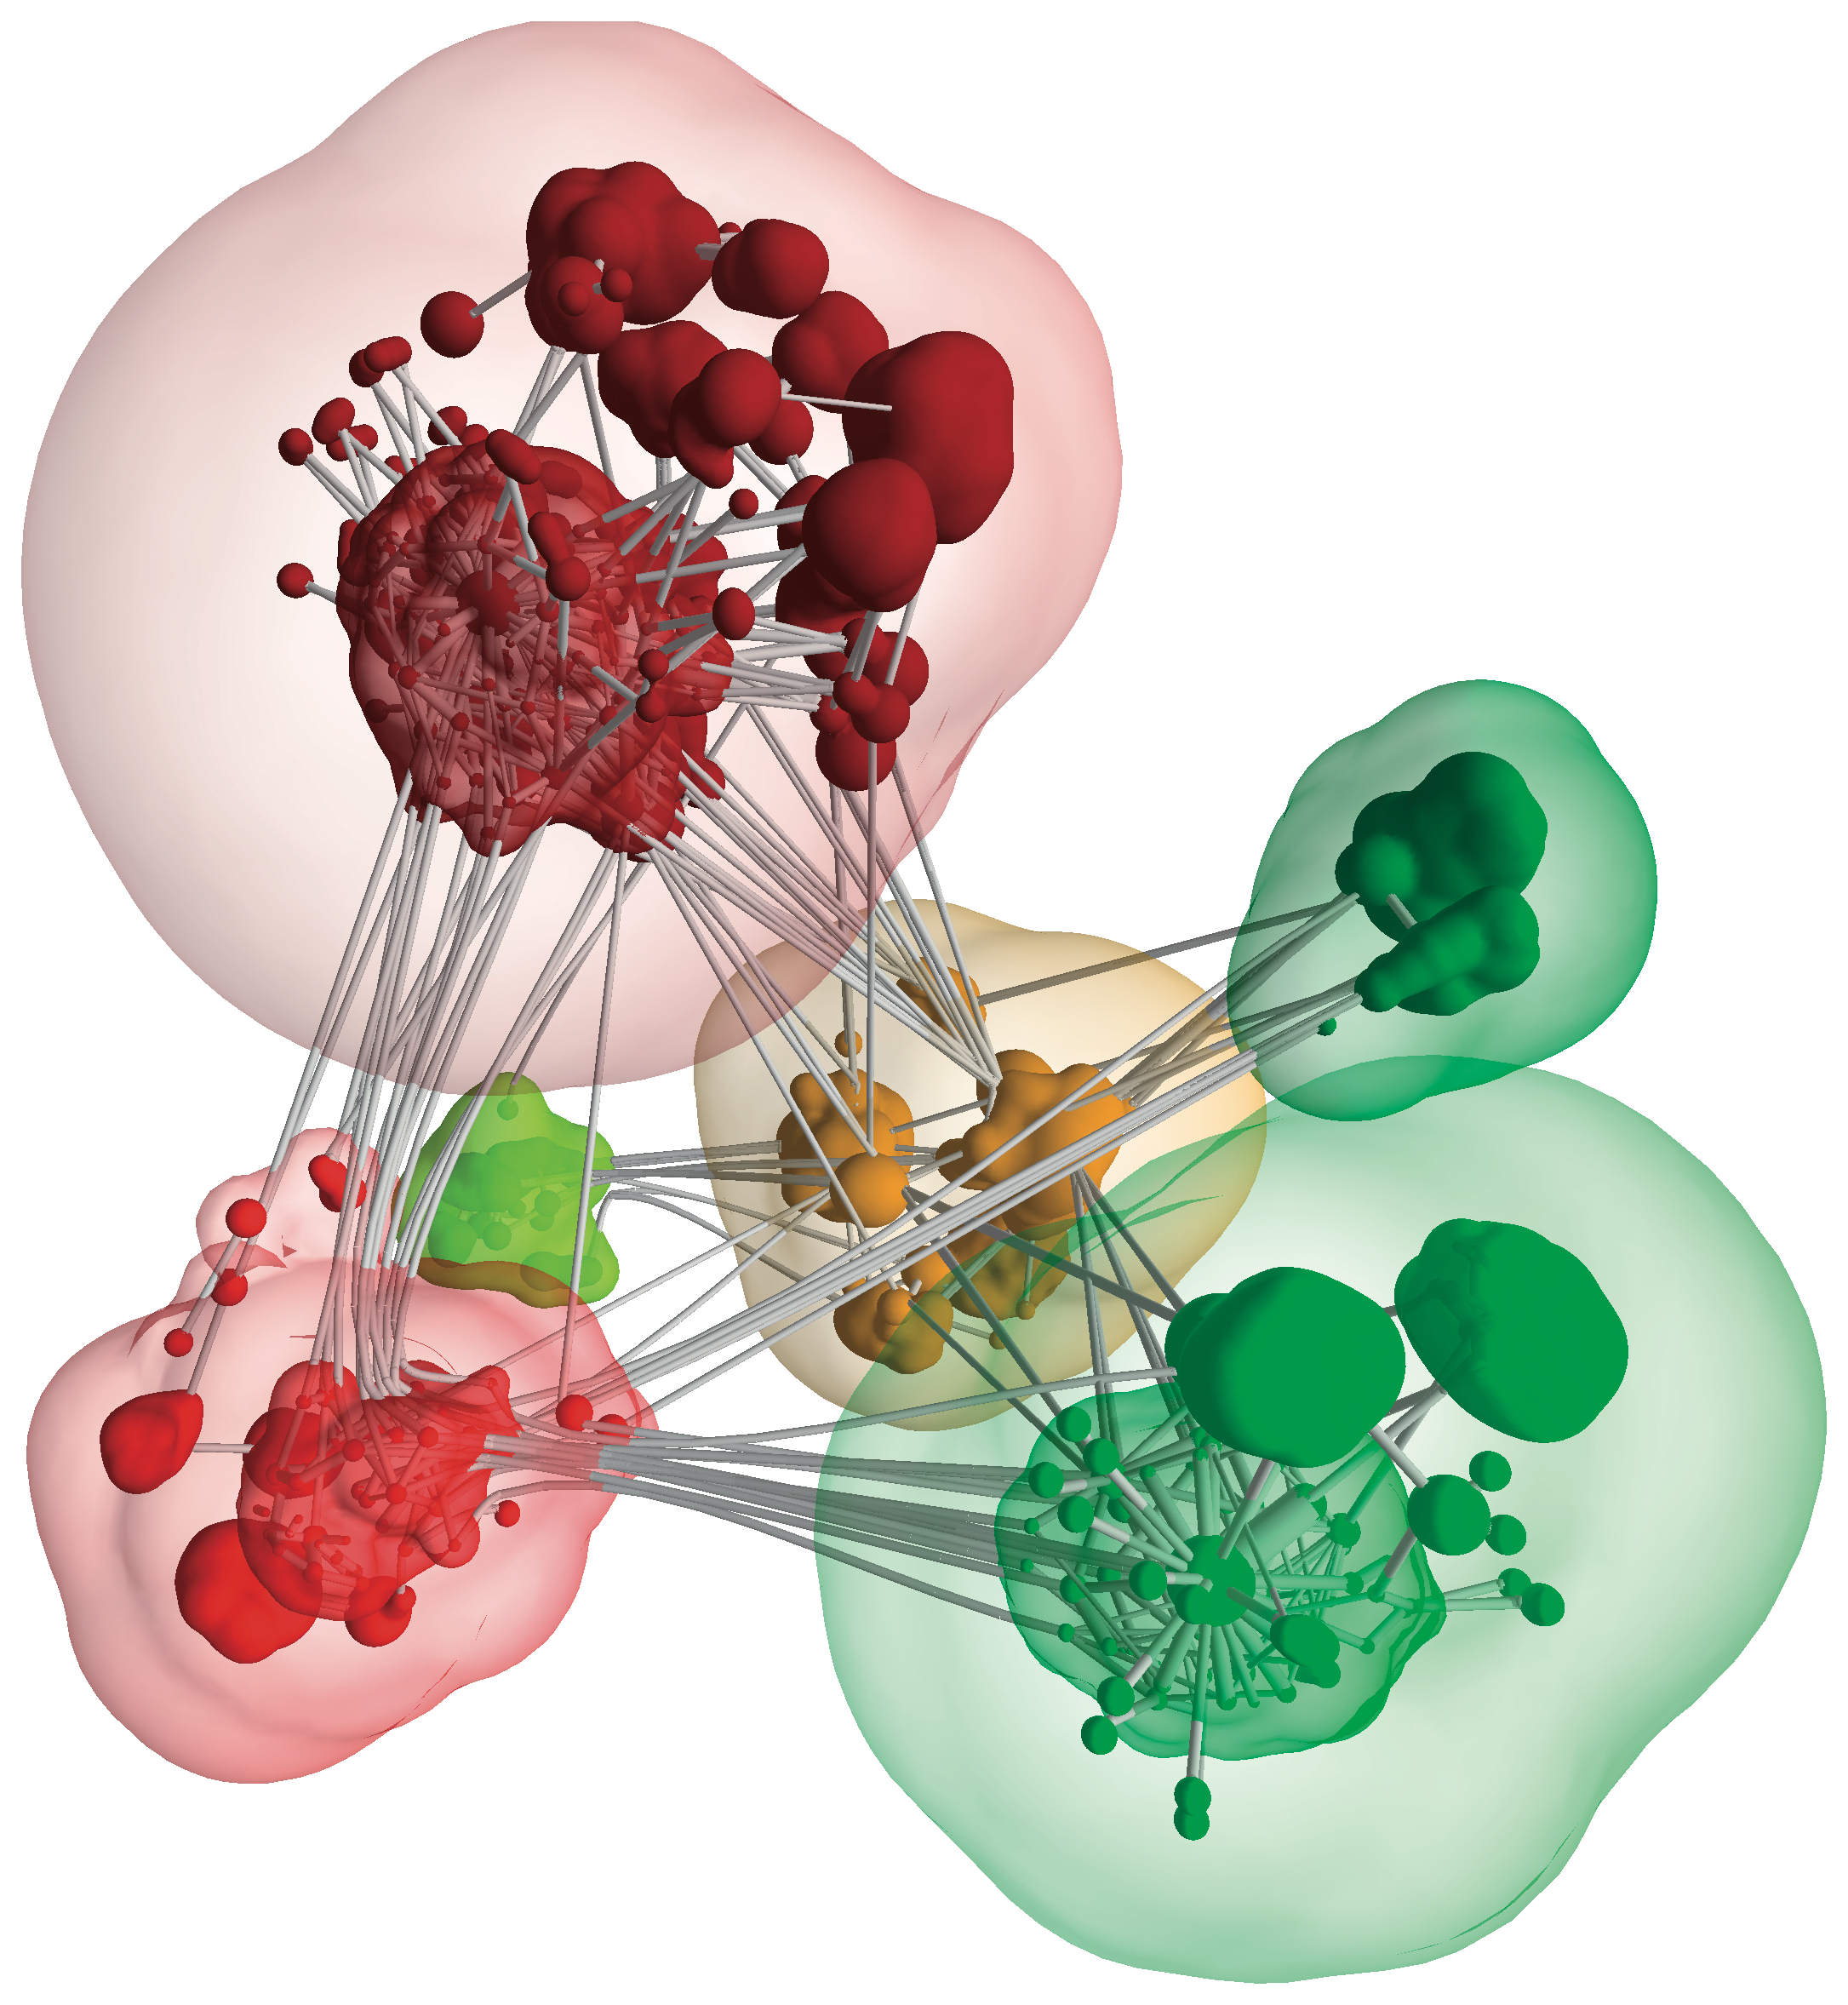
\includegraphics[width=\textwidth]{graphics/clusteredGraphVis.jpg}
        \subcaption{Visualization of a node-link dataset with multiple clusters from \cite{balzer_level--detail_2007}.}
        \label{fig:clusteredGraph}
    \end{subfigure}
    
    \caption[Optional caption for the figure list (often used to abbreviate long captions)]{Examples of multilayer visualizations.} % Remove the [...] argument if the original caption should be used in the figure list.
    \label{fig:relatedWorkExamples} 
  \end{figure}

\section{VR Visualizations}

\subsection{Layouts}

\subsubsection{Force based layout approaches}
In VR we see common 2D layout approaches like simple node-link diagrams adapted for the use in a 3D virtual scene. Often these layouts use a force based approach to calculate the node positions. 

Drogemuller\\
Examining virtual reality navigation techniques for 3D network visualisations\\
Uses a normal 3D node-link layout as a baseline.\\
\\
Sorger\\
Immersive Analytics of Large Dynamic Networks via Overview and Detail Navigation\\
3D force layout for node-link diagram\\
\\
Yang\\
Embodied Navigation in Immersive Abstract Data Visualization:
Is Overview+Detail or Zooming Better for 3D Scatterplot\\
uses 3D Scatterplot similar to node-link
\subsubsection{Constraint layout approaches}
Other concepts use fixed constrains to place their nodes and links.

Sorger\\
Fisheye Layout\\
Orig Paper https://vis.csh.ac.at/vrnetexplorer/\\
\\
Kwon\\
A Study of Layout, Rendering, and Interaction Methods for Immersive Graph Visualization\\
Spherical graph layouts, the viewer is placed at the center of the sphere, on which the graph is laid out.\\
\\
Halpin\\
Exploring Semantic Social Networks Using Virtual Reality\\
2D flat layout + use of extrusion
%Büschel\\
%Augmented Reality Graph Visualizations\\
%We present an exploration of the design space for edge styles and discuss the results of a user study comparing six different edge variants.\\
%\\
\\
\\
\\
\subsection{Navigation}
Content:
\begin{itemize}
    \item "Minimap"/Worlds-in-Miniature (WIM) in VR
    \item Scaling
    \item Room scale vs Table vs Seating
    \item Overview + Detail 
\end{itemize}
%In terms of navigation and interaction Yang et al. \cite{yang_embodied_2020} explored the possibility of zooming and rotation of an entire graph and Drogemuller \cite{drogemuller_examining_2020} compared different navigation concepts.\\
Papers: \\
Yang\\
Embodied Navigation in Immersive Abstract Data Visualization:
Is Overview+Detail or Zooming Better for 3D Scatterplot\\
\\
M Usoh\\
Walking > walking-in-place > flying, in virtual environments\\
\\
Zielasko\\
Remain seated: towards fully-immersive desktop VR\\
\\
Drogemuller\\
Examining virtual reality navigation techniques for 3D network visualisations\\
\\
Wolfgang Stuerzlinger\\
Simulated Reference Frame: A Cost-Effective Solution to Improve Spatial Orientation in VR\\
aka. Nintendo Wii Board Navigation\\
\\
Wolfgang Stuerzlinger\\
Evaluating Automatic Parameter Control Methods for Locomotion in Multiscale Virtual Environments\\
AUTOMATIC DISTANCE CONTROL teleporting\\

\subsection{Interaction}
Content: 
\begin{itemize}
    \item Edge Filtering
    \item Raycast/Laserpointer Selection
\end{itemize}

Drogemuller\\
VRige: Exploring Social Network Interactions in Immersive Virtual Environments\\
Raycast+Filter Cube\\
\\
Wolfgang Stürzlinger\\
Analyzing the Trade-off between Selection and Navigation in VR\\
\\
Yi-Jheng Huang\\
A gesture system for graph visualization in virtual reality environments\\
different hand gesture interactions\\
\\

%\subsection{Advantages of Visualization in VR}
%Kraus\\
%The Impact of Immersion on Cluster Identification Tasks\\
%quantitative user study to investigate the impact of immersion on cluster identification tasks in scatterplot visualizations\\
%\\
%Doug A. Bowman\\
%Virtual Reality: How Much Immersion Is Enough?\\
%\\
%M Cordeil\\
%Immersive Collaborative Analysis of Network Connectivity: CAVE-style or Head-Mounted Display?\\
%\\